\chapter{Построение черной дыры и загадка вблизи горизонта}

\lectureoverview{Мы построим черную дыру из трех частей: причинной диаграммы плоского пространства-времени, диаграммы Шварцшильда и теоремы Биркгофа для сферической оболочки. Эта конструкция показывает, что горизонт событий является глобальной границей и может начинаться в области, которая локально все еще плоская. Затем мы перейдем от причинной геометрии к энтропии и температуре Хокинга. Термометр, удерживаемый вблизи горизонта, становится сколь угодно горячим, тогда как свободно падающий наблюдатель не ожидает никакой локальной катастрофы. В заключительном рассуждении ставится вопрос о том, что именно может установить внешний эксперимент, не создавая при этом возмущения, которое он призван обнаружить.}

\section{Черная дыра при температуре пустого пространства}

Домашнее задание предполагалось такое: построить черную дыру и принести ее на занятие для показа и рассказа. Но ни у кого не нашлось ни одной для демонстрации, и более мягкую вводную задачу дал расчет, найденный через Wolfram. Какой радиус и масса дадут черной дыре температуру Хокинга, близкую к температуре космического микроволнового фона \(3\,\mathrm{K}\)?

\begin{classroomqa}
\audiencequestion{Что было вычислено на сайте?\lecturetimestamp{00:00:39}}
\lecturerresponse{Радиус черной дыры, температура которой составляет около \(3\,\mathrm{K}\). Смысл не в точном вычислении, а в оценке физического масштаба.}
\end{classroomqa}

Такая дыра на мгновение имела бы ту же температуру, что и ее окружение, но это равновесие было бы неустойчивым. Черная дыра Шварцшильда обладает отрицательной теплоемкостью. Если она становится чуть горячее тепловой ванны, она излучает, теряет массу и нагревается еще сильнее. Если она становится чуть холоднее, она поглощает, набирает массу и остывает еще сильнее.\editorialnote{Это и есть точный аргумент об устойчивости, стоящий за намеренно вольной аудиторной формулировкой. Канонический термостат не может обеспечить устойчивое равновесие для изолированной черной дыры Шварцшильда.}

Оценка начинается с характерной длины волны излучения при \(3\,\mathrm{K}\).

\begin{classroomqa}
\audiencequestion{Какая длина волны соответствует излучению с температурой около трех кельвинов?\lecturetimestamp{00:02:03}}
\lecturerresponse{В аудитории называли сантиметр, \(21\) сантиметр и даже \(10\) метров, прежде чем остановиться на микроволновом диапазоне. Полезным для этого рассуждения ответом по порядку величины был примерно сантиметр — достаточно мало, чтобы были уместны шутки про микроволновую печь и хлебницу.}
\end{classroomqa}

Типичный квант Хокинга имеет длину волны, сравнимую, с точностью до численных множителей, с радиусом Шварцшильда:
\begin{equation}
\lambda_{\mathrm{H}}\sim R_s,
\qquad
R_s=\frac{2GM}{c^2}.
\label{eq:l05-scale}
\end{equation}
Если взять использованное на лекции значение \(\lambda_{\mathrm H}\sim1\,\mathrm{cm}\), получаем \(R_s\sim1\,\mathrm{cm}\). Поскольку у черной дыры солнечной массы радиус составляет несколько километров, а \(R_s\) пропорционален \(M\), соответствующая масса примерно равна
\begin{equation}
M\sim10^{-5}M_\odot,
\label{eq:l05-rough-mass}
\end{equation}
что имеет планетный масштаб. Поэтому на лекции получается оценка земного масштаба.

\begin{classroomqa}
\audiencequestion{Согласуется ли это с численным результатом из Wolfram?\lecturetimestamp{00:05:53}}
\lecturerresponse{Сообщенный результат был ближе к массе Луны. По сравнению с грубой оценкой это казалось малым, но любой из ответов подчеркивает задуманный смысл: этот объект не из тех, что можно носить в кармане.}
\end{classroomqa}

Если сохранить константы, расхождение становится понятным. Из
\begin{equation}
T_H=\frac{\hbar c}{4\pi k_B R_s},
\end{equation}
при \(T_H=3\,\mathrm{K}\) получаем
\begin{equation}
R_s\simeq6.1\times10^{-5}\,\mathrm{m},
\qquad
M\simeq4.1\times10^{22}\,\mathrm{kg}.
\label{eq:l05-three-kelvin}
\end{equation}
Это соответствует скорее лунной, чем земной массе. Микроволновая длина волны, множитель \(4\pi\) и выбор того, какую длину волны чернотельного излучения считать типичной, объясняют разрыв между быстрой оценкой и численным значением.\editorialnote{Уравнение~\eqref{eq:l05-three-kelvin} восстанавливает численные множители, опущенные в размерностной оценке на лекции. Сама эта оценка сохранена, потому что именно таким путем шли в аудитории.}

Эти вычисления выполнили свою задачу. Теперь мы хотим построить черную дыру — математически и в воображении. Полные уравнения поля для нашей нынешней цели слишком сложны. Основные факты нам дадут рисунки.

\section{Первая рабочая часть: плоское пространство-время}

Используем полярные координаты с центром в точке наблюдателя и опустим углы. Приведенные координаты — это \((t,r)\), где \(r\geq0\). Точка на этой приведенной диаграмме не является точкой четырехмерного пространства-времени; кроме случая \(r=0\), она представляет целую сферу \(S^2\).

Радиальные световые лучи движутся под углом \(45^\circ\). Входящий луч достигает начала координат, а исходящий покидает его вдоль другого нулевого направления. Бесконечную полуплоскость можно сжать в конечный клин Пенроуза с помощью конформного преобразования. Оно не единственно. Существенно то, что бесконечность переносится на конечную границу, а радиальные нулевые направления остаются под углом \(45^\circ\). Если говорить так, как у доски, мы сплющиваем диаграмму.

\begin{figure}[htbp]
\centering
\includegraphics[width=0.68\textwidth]{lecture_05_figure_02.png}
\caption{Верхняя половина компактифицированного радиального пространства-времени Минковского. Вертикальная граница — \(r=0\), а семейства кривых сгущаются к компактифицированной бесконечности.}
\lectureframe{00:11:41.560}
\end{figure}

\begin{figure}[htbp]
\centering
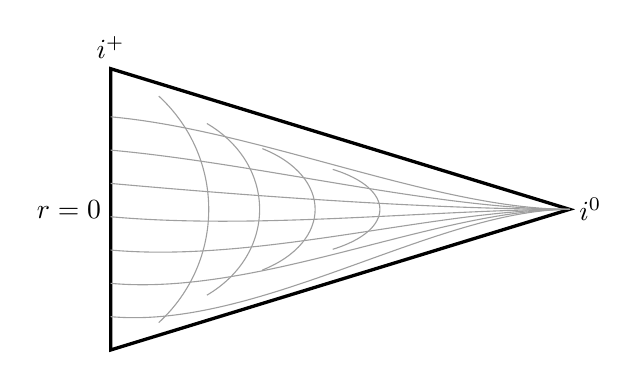
\begin{tikzpicture}[scale=0.94]
\coordinate (O) at (0,0);
\coordinate (P) at (0,3.8);
\coordinate (I) at (6.2,1.9);
\draw[very thick] (O)--(P)--(I)--cycle;
\foreach \y in {0.45,0.90,1.35,1.80,2.25,2.70,3.15} {
  \draw[gray!75] (0,\y) .. controls (2.0,\y-0.18) and (4.4,1.9) .. (I);
}
\draw[gray!75] (0.65,0.37) .. controls (1.55,1.20) and (1.55,2.60) .. (0.65,3.43);
\draw[gray!75] (1.30,0.74) .. controls (2.25,1.30) and (2.25,2.50) .. (1.30,3.06);
\draw[gray!75] (2.05,1.08) .. controls (3.00,1.46) and (3.00,2.34) .. (2.05,2.72);
\draw[gray!75] (3.00,1.36) .. controls (3.85,1.62) and (3.85,2.18) .. (3.00,2.44);
\node[left] at (0,1.9) {\(r=0\)};
\node[above] at (P) {\(i^+\)};
\node[right] at (I) {\(i^0\)};
\end{tikzpicture}
\caption{Аккуратный вариант верхнего клина. Кривые — это качественные семейства при постоянных \(r\) и постоянных \(t\), а не точная координатная сетка.}
\label{fig:l05-flat-wedge}
\end{figure}

Мировые линии при фиксированном \(r\), вертикальные до компактификации, выгибаются и сгущаются вблизи будущей времениподобной бесконечности. Срезы при постоянном \(t\) точно так же сгущаются к пространственной бесконечности. Это сгущение является координатным эффектом, а не физическим сжатием вещества.

Правило \(45^\circ\) непосредственно применимо к радиальному свету. Луч с угловым моментом может не попасть в начало координат, достичь ненулевого расстояния наибольшего сближения и вернуться наружу. Вдали от начала координат его проекция выглядит почти радиальной; лишь вблизи точки наибольшего сближения траектория в приведенных координатах \((t,r)\) заметно искривляется. Этим первая рабочая часть завершена.

\section{Вторая рабочая часть: вечный Шварцшильд}

Максимально продолженное решение Шварцшильда содержит два внешних ромба, будущую область черной дыры и прошлую область белой дыры. Его верхняя и нижняя волнистые границы — будущая и прошлая сингулярности. Для черной дыры, образованной коллапсом, большая часть этой структуры вскоре будет отброшена, но обычная правая внешняя область — как раз тот фрагмент, который нам нужен.

\begin{figure}[htbp]
\centering
\includegraphics[width=0.72\textwidth]{lecture_05_figure_03.png}
\caption{Диаграмма вечного Шварцшильда, где справа показаны обычная внешняя область и ее схематическая координатная сетка.}
\lectureframe{00:16:55.975}
\end{figure}

\begin{figure}[htbp]
\centering
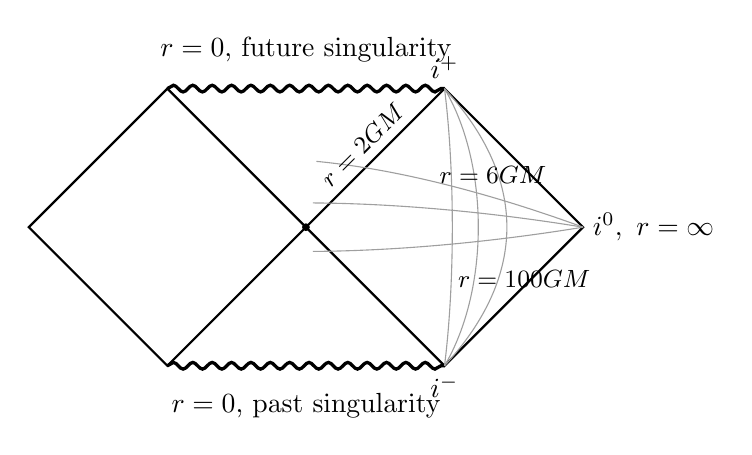
\begin{tikzpicture}[scale=0.88]
\coordinate (C) at (0,0);
\coordinate (TL) at (-2.0,2.0);
\coordinate (L) at (-4.0,0);
\coordinate (BL) at (-2.0,-2.0);
\coordinate (TR) at (2.0,2.0);
\coordinate (R) at (4.0,0);
\coordinate (BR) at (2.0,-2.0);
\draw[thick] (C)--(TL)--(L)--(BL)--(C);
\draw[thick] (C)--(TR)--(R)--(BR)--(C);
\draw[very thick,decorate,decoration={snake,amplitude=1.2pt,segment length=7pt}] (TL)--(TR);
\draw[very thick,decorate,decoration={snake,amplitude=1.2pt,segment length=7pt}] (BL)--(BR);
\draw[gray!75] (TR) .. controls (2.15,0.8) and (2.15,-0.8) .. (BR);
\draw[gray!75] (TR) .. controls (2.65,0.9) and (2.65,-0.9) .. (BR);
\draw[gray!75] (TR) .. controls (3.20,0.7) and (3.20,-0.7) .. (BR);
\draw[gray!75] (0.15,0.95) .. controls (1.5,0.82) and (2.9,0.40) .. (R);
\draw[gray!75] (0.10,0.35) .. controls (1.5,0.34) and (2.9,0.18) .. (R);
\draw[gray!75] (0.10,-0.35) .. controls (1.5,-0.34) and (2.9,-0.18) .. (R);
\fill (C) circle (1.6pt);
\node[above] at (TR) {\(i^+\)};
\node[below] at (BR) {\(i^-\)};
\node[right] at (R) {\(i^0,\ r=\infty\)};
\node[above] at (0,2.25) {\(r=0\), future singularity};
\node[below] at (0,-2.25) {\(r=0\), past singularity};
\node[rotate=45,above,font=\small] at (1.0,1.0) {\(r=2GM\)};
\node[font=\small] at (2.70,0.75) {\(r=6GM\)};
\node[font=\small] at (3.15,-0.75) {\(r=100GM\)};
\end{tikzpicture}
\caption{Правая внешняя область при больших радиусах напоминает плоский клин. Ее внутренняя светоподобная граница — это \(r=2GM\) при \(c=1\); остальные подписанные радиусы являются лишь схематическими примерами.}
\label{fig:l05-eternal-schwarzschild}
\end{figure}

Вдали от дыры внешняя область все больше напоминает компактифицированное плоское пространство-время. Линии вроде \(r=6GM\) и \(r=100GM\) все ближе подходят к поведению обычных мировых линий постоянного радиуса. Внутренняя граница внешней области находится при
\begin{equation}
r=2GM
\end{equation}
в единицах \(c=1\).

Вблизи центра сравнение с плоским пространством перестает работать. Радиальный луч в пространстве Минковского достигает \(r=0\) и вновь выходит с противоположной физической стороны. Луч, направленный в будущее, внутри области Шварцшильда не отскакивает. Он оканчивается на пространственноподобной сингулярности при \(r=0\). Именно это причинное различие должна сохранить конструкция коллапса.

\section{Теорема, позволяющая склеить части}

Недостающий элемент впервые появляется в ньютоновской гравитации. Для сферически-симметричного распределения массы закон Гаусса дает
\begin{equation}
\oint\mathbf g\cdot d\mathbf A=-4\pi G M_{\mathrm{enc}},
\end{equation}
и, следовательно,
\begin{equation}
\mathbf g(r)=-\frac{G M_{\mathrm{enc}}(r)}{r^2}\,\hat{\mathbf r}.
\label{eq:l05-shell-theorem}
\end{equation}
Материя вне сферы радиуса \(r\) не вносит туда никакого суммарного поля. Для полой оболочки полной массы \(M\),
\begin{equation}
\mathbf g=
\begin{cases}
0, & r<R_{\mathrm{shell}},\\[3pt]
-\dfrac{GM}{r^2}\hat{\mathbf r}, & r>R_{\mathrm{shell}}.
\end{cases}
\end{equation}

Теорема Биркгофа — релятивистский аналог. Любая сферически-симметричная вакуумная область локально является областью Шварцшильда с постоянным массовым параметром. Пустая внутренняя область сферической оболочки имеет нулевой массовый параметр и локально является пространством Минковского; внешняя область имеет массовый параметр \(M\) и описывается решением Шварцшильда:
\begin{equation}
\begin{aligned}
M_{\mathrm{enc}}&=0 && \text{inside the shell},\\
M_{\mathrm{enc}}&=M && \text{outside the shell}.
\end{aligned}
\label{eq:l05-birkhoff}
\end{equation}
Это утверждение остается полезным и при движении оболочки, потому что вакуумные области по обе стороны от нее сохраняют сферическую симметрию.

\editorialnote{То, что внутри плоско, — локальное утверждение. Статическая оболочка может изменить нормировку внутренней временной координаты, хотя внутренняя кривизна и равна нулю. Для движущейся или светоподобной оболочки две вакуумные метрики должны быть согласованы на оболочке; в идеализации это склейка по тонкой оболочке, тесно связанная с входящей геометрией Vaidya. Ни одно из этих уточнений не меняет причинного аргумента с вырезанием и склейкой, используемого здесь.}

Для лабораторной наглядности представьте себе сферу, густо покрытую синхронизированными лазерами, как на крупной установке инерциального удержания, причем все они одновременно посылают свет внутрь. В идеализации нет никакой аппаратуры, есть лишь идеально сферическая световая оболочка. Оболочка несет энергию \(E\), поэтому внешний массовый параметр равен
\begin{equation}
M=\frac{E}{c^2},
\end{equation}
или просто \(E=M\) в естественных единицах. Поскольку оболочка движется со скоростью света, на приведенной диаграмме она является входящей светоподобной линией. Каждая точка на этой линии представляет целый сферический волновой фронт, а не траекторию одного фотона.

\section{Сшивание пространства-времени коллапса}

Начнём с плоского пространства-времени и изобразим входящую светоподобную оболочку. Область внутри неё верна: теорема Биркгофа утверждает, что она плоская. Область снаружи неверна, потому что внешняя область уже должна учитывать полную массу оболочки через свою геометрию Шварцшильда.

Теперь изобразим ту же оболочку на диаграмме вечного решения Шварцшильда. Здесь область вне неё верна. Белая дыра, вторая внешняя область и неподходящая часть внутренней области чёрной дыры неверны для коллапса, начинающегося в обычном пустом пространстве, поэтому сотрём их.

\begin{figure}[htbp]
\centering
\includegraphics[width=0.72\textwidth]{lecture_05_figure_05.png}
\caption{Светоподобная оболочка, показанная красным, проведена через диаграмму Шварцшильда, при этом выделяется правильная внешняя область.}
\lectureframe{00:32:00.000}
\end{figure}

В плоском фрагменте оболочка достигает \(r=0\). В шварцшильдовском фрагменте она достигает начала будущей сингулярности. Это одна и та же конечная точка. Склеивание плоской внутренней области со шварцшильдовской внешней областью вдоль оболочки даёт простейшее пространство-время, описывающее образование чёрной дыры.

\begin{classroomqa}
\audiencequestion{В верхней левой точке склейки действительно ли конечная точка в плоском пространстве совпадает с точкой на стороне Шварцшильда?\lecturetimestamp{00:34:50}}
\lecturerresponse{Да. Оболочка в плоском пространстве сжимается до \(r=0\), и сингулярность Шварцшильда также находится при \(r=0\). Две отождествляемые точки имеют один и тот же геометрический смысл: двусфера сжалась до нулевого размера.}
\end{classroomqa}

\begin{figure}[htbp]
\centering
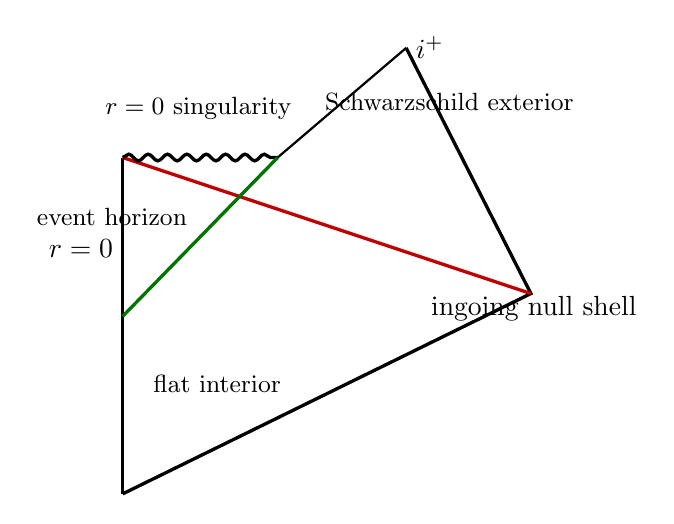
\begin{tikzpicture}[scale=0.96]
\coordinate (A) at (0,-2.8);
\coordinate (B) at (0,1.65);
\coordinate (C) at (2.05,1.65);
\coordinate (D) at (5.4,-0.15);
\coordinate (E) at (3.75,3.10);
\coordinate (H0) at (0,-0.45);
\draw[very thick] (A)--(B);
\draw[very thick] (A)--(D)--(E);
\draw[very thick,red!75!black] (D)--(B);
\draw[very thick,decorate,decoration={snake,amplitude=1.2pt,segment length=7pt}] (B)--(C);
\draw[very thick,green!45!black] (H0)--(C);
\draw[thick] (C)--(E);
\node[left] at (0,0.45) {\(r=0\)};
\node[below right] at (3.95,-0.05) {ingoing null shell};
\node[font=\small] at (1.25,-1.35) {flat interior};
\node[font=\small,anchor=west] at (2.55,2.38) {Schwarzschild exterior};
\node[above,font=\small] at (1.0,2.02) {\(r=0\) singularity};
\node[above left,font=\small] at (0.98,0.62) {event horizon};
\node[right] at (E) {\(i^+\)};
\end{tikzpicture}
\caption{Геометрия коллапса. Красная оболочка соединяет плоскую внутреннюю область со шварцшильдовской внешней. Зелёный горизонт событий начинается раньше в плоской области и оканчивается на будущей границе области чёрной дыры.}
\label{fig:l05-collapse}
\end{figure}

Эта конструкция отвечает на вопрос, оставшийся после вечного решения. Чёрная дыра, возникшая при коллапсе, не имеет ни прошлой белой дыры, ни второй асимптотической вселенной. При этом у неё всё же есть будущая сингулярность.

\section{Горизонт — глобальная граница}

Старое обозначение \(r=2GM\) указывало горизонт в стационарной геометрии Шварцшильда, но это не то определение, которое требуется в динамическом пространстве-времени.

\begin{definition}
Будущий горизонт событий — это граница множества событий, из которых можно послать причинный сигнал, направленный в будущее, на будущую нулевую бесконечность.
\end{definition}

На диаграмме коллапса проследите исходящий светоподобный луч, которому как раз не удаётся уйти на бесконечность. Лучи чуть снаружи от него достигают бесконечности; лучи чуть внутри него оканчиваются на сингулярности. Эта разделяющая линия и есть истинный горизонт.

\begin{figure}[htbp]
\centering
\includegraphics[width=0.72\textwidth]{lecture_05_figure_06.png}
\caption{Завершённое построение на доске. Входящая оболочка показана красным, а горизонт событий — зелёным; часть зелёной линии лежит в ещё плоской области под оболочкой.}
\lectureframe{00:39:10.000}
\end{figure}

Поразительная особенность теперь уже неизбежна. Горизонт простирается назад в область, куда оболочка ещё не пришла. Геометрия там локально плоская, и наблюдатель, пересекающий эту линию, не обнаруживает никакого импульса кривизны, стены или вспышки. Тем не менее он уже не может достичь бесконечности, поскольку будущая оболочка перекроет любой возможный путь к спасению. Горизонты событий телеологичны именно в этом глобальном смысле: для определения положения такого горизонта нужно знать всё будущее пространства-времени.\editorialnote{Никакой локальный эксперимент не может установить, что только что был пересечён гладкий горизонт событий. Другие понятия, такие как кажущийся или ловушечный горизонты, более локальны и во время коллапса не обязаны совпадать с горизонтом событий.}

Аналогия со сливом выделяет причинную идею. Представьте гребца возле слива, закрытого пробкой, в неподвижном озере. Если бы пробка оставалась на месте вечно, гребец мог бы уплыть. Если же наверняка известно, что кто-то её вытащит, то последующее течение может сделать уход невозможным, хотя вода пока ещё не движется. Замёрзшая Ниагара показывает то же самое: спокойная вода не гарантирует будущего пути к безопасности.

\begin{classroomqa}
\audiencequestion{Пробку выдёргивают потому, что сферическая оболочка света становится всё более концентрированной?\lecturetimestamp{00:43:13}}
\lecturerresponse{Концентрация создаёт чёрную дыру, но история со сливом используется для более узкой цели: можно уже оказаться по ту сторону точки невозврата ещё до того, как локально произойдёт что-либо драматическое.}
\end{classroomqa}

\subsection{Горизонт из растущих сфер}

Каждая точка редуцированного горизонта представляет \(S^2\). В первой точке горизонта эта сфера имеет нулевую площадь. Поднимаясь вверх вдоль него, она растёт, пока её ареальный радиус не достигает
\begin{equation}
R_s=\frac{2GM}{c^2}.
\end{equation}
Для стационарной дыры он остаётся таким, а если внутрь падает ещё энергия, то снова растёт.

\editorialnote{В идеализированной диаграмме сферического коллапса образующие горизонта встречаются в точке образования, или складке, при \(r=0\). Нулевую площадь имеет именно эта предельная двусфера; это утверждение не следует понимать так, будто конечный горизонт Шварцшильда внезапно сжимается в точку.}

\subsection{Что может восстановить далёкий наблюдатель}

Далее следует длинное обсуждение, в котором различаются наблюдатель, уже находящийся внутри глобального горизонта, и история того, как он там оказался.

\begin{classroomqa}
\audiencequestion{Каково положение человека, оказавшегося в ловушке до прихода оболочки? С точки зрения далёкого наблюдателя, находится ли он вне горизонта?\lecturetimestamp{00:44:03}}
\lecturerresponse{Нет. Как только мировая линия оказывается за горизонтом событий, её будущее оканчивается на сингулярности, и никакой новый сигнал от неё не достигает далёкого наблюдателя. Однако существование этого человека там не началось. Более ранние частицы, предки или иная предшествующая энергия пришли из области, которая была видима.}
\end{classroomqa}

Поэтому далёкий наблюдатель может видеть, как предшествующее вещество приближается к горизонту, ни разу не получая сигнала из-за него. Нет никакого противоречия в том, чтобы видеть сквозь входящую оболочку: она состоит из света, и наблюдатель может также видеть саму оболочку и сделать вывод, что образовалась чёрная дыра.

\begin{classroomqa}
\audiencequestion{Проходит ли линия зрения через коллапсирующую оболочку, и может ли внешний наблюдатель всё же знать, что чёрная дыра образовалась?\lecturetimestamp{00:46:51}}
\lecturerresponse{Да. Наблюдатель видит входящую оболочку и может принимать свет, траектория которого пересекает её, пока этот свет ещё способен уйти. Странным выглядит то, что предшествующее вещество приближается к только что определённому горизонту ещё до того, как оболочка достигает центра.}
\end{classroomqa}

\begin{classroomqa}
\audiencequestion{Остаётся ли в силе правило, что снаружи вещество выглядит так, словно оно сжато на горизонте?\lecturetimestamp{00:47:49}}
\lecturerresponse{Да. Во внешнем описании оно остаётся связанным с горизонтом, испытывая всё больший красный сдвиг, пока более поздний квантовый процесс испарения чёрной дыры не меняет картину.}
\end{classroomqa}

Это внешнее описание подводит к следующей теме. Если информация кажется нанесённой на двумерную поверхность, то уже не так удивительно, что энтропия чёрной дыры пропорциональна площади этой поверхности.

\section{Энтропия и температура, наблюдаемая с бесконечности}

Вблизи большого горизонта мы можем заменить сферическую поверхность локальной плоскостью, подобно тому как в небольшой лаборатории пользуемся приближением плоской Земли. Тогда можно свести вместе два факта из предыдущего обсуждения:
\begin{equation}
\begin{aligned}
S_{\mathrm{BH}}&\propto A_H,\\
\Delta A_H&\sim \ell_P^2
\quad\text{per added bit, schematically}.
\end{aligned}
\end{equation}
Мнемоническое правило один бит на планковскую площадь выражает закон площади; это не микроскопический вывод.

Температура Хокинга, измеряемая далеко от чёрной дыры Шварцшильда, равна
\begin{equation}
T_H=\frac{\hbar c^3}{8\pi GMk_B}.
\label{eq:l05-hawking}
\end{equation}
С учётом \(R_s=2GM/c^2\),
\begin{equation}
T_H=\frac{\hbar c}{4\pi k_B R_s}.
\label{eq:l05-hawking-radius}
\end{equation}
Следовательно, более крупные дыры холоднее.

\begin{classroomqa}
\audiencequestion{Может ли температура зависеть от положения?\lecturetimestamp{00:52:43}}
\lecturerresponse{В обычном разговоре, конечно, может: в Нью-Йорке и Стэнфорде вовсе не обязана быть одна и та же температура. Более точный вопрос касается системы в гравитационном тепловом равновесии. Там показания локальных термометров могут меняться с высотой, хотя равновесная температура с учётом красного смещения постоянна.}
\end{classroomqa}

Температуру считывают по локальным кинетическим энергиям. В разреженной атмосфере над нагретой Землёй молекулы теряют кинетическую энергию, поднимаясь, и приобретают её, опускаясь. Фотоны при движении вверх испытывают красное смещение, а вниз — синее. Поэтому термометр внизу и термометр вверху не обязаны показывать одну и ту же локальную шкалу энергий.

Для статического пространства-времени соотношение равновесия имеет вид
\begin{equation}
T_{\mathrm{loc}}(r)\sqrt{-g_{tt}(r)}=T_\infty,
\label{eq:l05-tolman}
\end{equation}
это закон Толмена. Температура Хокинга в уравнении~\eqref{eq:l05-hawking} — это \(T_\infty\), показание, нормированное на бесконечности.

\section{Горячая статическая атмосфера у горизонта}

Пусть \(\rho\) — собственное расстояние, отсчитываемое наружу от горизонта. Вблизи большого горизонта Шварцшильда уравнение~\eqref{eq:l05-tolman} принимает вид
\begin{equation}
k_B T_{\mathrm{loc}}(\rho)
\simeq\frac{\hbar c}{2\pi\rho},
\label{eq:l05-local-temperature-si}
\end{equation}
или, в единицах \(c=\hbar=k_B=1\),
\begin{equation}
T_{\mathrm{loc}}(\rho)=\frac{1}{2\pi\rho}.
\label{eq:l05-local-temperature}
\end{equation}

\begin{figure}[htbp]
\centering
\includegraphics[width=0.72\textwidth]{lecture_05_figure_07.png}
\caption{Асимптотическая температура Хокинга и локальная температура у горизонта \(T(\rho)=1/(2\pi\rho)\), записанные на доске.}
\lectureframe{01:02:40.000}
\end{figure}

Маленький термометр, удерживаемый на тросе при фиксированном \(\rho\), показывает всё более высокую температуру по мере опускания. Атом, удерживаемый в этой статической атмосфере, сначала возбуждается, затем ионизуется, затем распадается; при ещё больших локальных энергиях даже ядра и адроны перестают сохранять целостность. Если опускать человека ногами вперёд, получается запоминающийся диагноз: горячая ступня.

Слово \emph{held} существенно. Эта расходимость относится к детектору, удерживаемому неподвижным ускорением. Она описывает тепловую атмосферу, красносмещённую относительно внешнего времени. Свободно падающий детектор движется по другой траектории и для достаточно большой дыры в регулярном квантовом состоянии не обязан встретить на горизонте расходящуюся тепловую ванну.\editorialnote{Это различие отделяет температуру Толмана и температуру ускорения, наблюдаемые статическими наблюдателями, от регулярного локального опыта свободно падающего наблюдателя. В лекции этот контраст намеренно превращается в операционную загадку, а не снимается одной лишь терминологией.}

Порог ионизации делает конфликт конкретным.

\begin{classroomqa}
\audiencequestion{Сколько энергии требуется для ионизации водорода?\lecturetimestamp{01:06:53}}
\lecturerresponse{Слушатели называют \(13\) электрон-вольт, правильно указывая \(13.6\,\mathrm{eV}\) как энергию ионизации основного состояния. Сопутствующая оценка в несколько тысяч кельвинов слишком мала, но для аргумента требуется лишь существование конечного порога.}
\end{classroomqa}

Действительно,
\begin{equation}
\frac{13.6\,\mathrm{eV}}{k_B}\simeq1.58\times10^5\,\mathrm{K}.
\end{equation}
Следовательно, существует некоторое малое собственное расстояние \(\rho_{\mathrm{ion}}\), на котором статическая температура достигает масштаба ионизации. Статическая экстраполяция утверждает, что атом должен быть уже ионизован там, снаружи горизонта. Свободно падающий атом, напротив, не ожидает никакой локальной стенки и может пересечь горизонт за конечное собственное время. Может ли внешний наблюдатель провести эксперимент, который позволит сделать выбор между этими описаниями?

\section{Микроскоп Гейзенберга}

Прежде чем применять этот вопрос к чёрной дыре, вспомним фотонный микроскоп. Чтобы локализовать частицу с разрешением \(\Delta x\), длина волны зонда должна удовлетворять
\begin{equation}
\lambda\lesssim\Delta x.
\end{equation}
Тогда один фотон несёт импульс не меньше
\begin{equation}
p_\gamma\gtrsim\frac{\hbar}{\Delta x}.
\label{eq:l05-microscope}
\end{equation}
Рассеяние этого фотона создаёт отдачу того же порядка. Если сначала измерить положение, а затем немедленно проверить скорость, во втором измерении обнаружится состояние, изменённое первым. Эксперимент создаёт условие, которое он и был призван исключить.

\begin{figure}[htbp]
\centering
\includegraphics[width=0.70\textwidth]{lecture_05_figure_08.png}
\caption{Микроскоп даёт оценки \(\Delta x\gtrsim\lambda\) и \(p_\gamma\gtrsim\hbar/\Delta x\).}
\lectureframe{01:11:50.000}
\end{figure}

Это не просто ограничение классической оптики. Классические волны можно было бы делать сколь угодно слабыми; квантовая механика требует по меньшей мере одного кванта в событии успешной регистрации. Поэтому улучшение пространственного разрешения неизбежно влечёт за собой конечную передачу импульса.

\section{Эксперимент вблизи горизонта}

Теперь пусть атом падает через слой, начинающийся на \(\rho_{\mathrm{ion}}\). Относительно статической системы отсчёта он движется внутрь почти со скоростью \(c\), так что доступный интервал до пересечения горизонта имеет порядок
\begin{equation}
\Delta\tau\sim\frac{\rho_{\mathrm{ion}}}{c}.
\label{eq:l05-fall-time}
\end{equation}
После пересечения никакой результат уже нельзя передать обратно наружу. За этот короткий интервал измерение должно отличить неионизованный атом от ионизованного.

Чтобы пространственно разрешить атом внутри этого слоя, требуется
\begin{equation}
\lambda\lesssim\rho_{\mathrm{ion}}.
\end{equation}
Соответственно, энергия зонда ограничена снизу:
\begin{equation}
E_\gamma=cp_\gamma
\gtrsim\frac{\hbar c}{\rho_{\mathrm{ion}}}.
\label{eq:l05-probe-energy}
\end{equation}
За исключением множителя \(2\pi\), это тот же масштаб, что и в уравнении~\eqref{eq:l05-local-temperature-si}:
\begin{equation}
E_\gamma\gtrsim2\pi k_B T_{\mathrm{loc}}(\rho_{\mathrm{ion}}).
\label{eq:l05-probe-temperature}
\end{equation}
Фотон, достаточно энергичный, чтобы разрешить событие, также достаточно энергичен, чтобы ионизовать атом.

\begin{figure}[htbp]
\centering
\includegraphics[width=0.72\textwidth]{lecture_05_figure_09.png}
\caption{Пригоризонтная оценка на доске: условие \(\lambda<\rho\) требует локальной энергии зонда порядка \(\hbar c/\rho\).}
\lectureframe{01:18:30.000}
\end{figure}

\begin{classroomqa}
\audiencequestion{Ионизует ли этот высокоэнергетический фотон атом даже в его свободно падающей системе отсчёта?\lecturetimestamp{01:19:07}}
\lecturerresponse{Да. В атом попадает реальный энергичный квант, и в своей собственной локальной системе отсчёта он получает отдачу или ионизуется. Измерение не выявляет невозмущённое падение; оно заменяет его возмущённым.}
\end{classroomqa}

\begin{classroomqa}
\audiencequestion{Что, если атом просто падает и никто не проводит эксперимент?\lecturetimestamp{01:19:39}}
\lecturerresponse{Тогда именно это возмущение отсутствует. Если внешний наблюдатель всё же проводит эксперимент с высоким разрешением, атому приходится плохо. Аргумент касается того, что можно проверить снаружи, а не доказательства того, что неизмеренный падающий объект сгорает.}
\end{classroomqa}

\subsection{Могут ли термометр или передатчик справиться лучше?}

Перемещение аппаратуры не устраняет информационную проблему.

\begin{classroomqa}
\audiencequestion{Нельзя ли провести измерение дальше, восстановить градиент или позволить свободно падающему термометру записать температуру, а потом извлечь эту запись?\lecturetimestamp{01:19:51}}
\lecturerresponse{Чтобы узнать пригоризонтную запись, что-то должно взаимодействовать с термометром и вернуть информацию в виде квантов. Чтобы развернуть термометр обратно, требуется сильное ускорение, тогда как считывание его на расстоянии требует излучения или рассеяния. Любой из этих путей изменяет физическую систему, чью невозмущённую историю и предполагалось проверить.}
\end{classroomqa}

\begin{classroomqa}
\audiencequestion{Является ли необходимость высокой энергии зонда при малом разрешении той же самой трудностью, что и вывод отражённого сигнала из пригоризонтной области?\lecturetimestamp{01:21:51}}
\lecturerresponse{Это две стороны одного и того же красносмещённого масштаба. Фотон может иметь малую энергию, когда наконец достигает бесконечности, потому что при выходе наружу он теряет энергию, но там, где он разрешает атом, его локальная частота должна быть высокой.}
\end{classroomqa}

\editorialnote{Фотон, испущенный непосредственно вне горизонта, не обязан обладать большой энергией лишь для того, чтобы выбраться наружу. Решающее требование здесь состоит в том, чтобы он закодировал событие в течение собственного времени и на собственном расстоянии порядка \(\rho\); гравитационное красное смещение затем связывает эту большую локальную частоту с гораздо меньшей асимптотической.}

\begin{classroomqa}
\audiencequestion{Может ли объект сам испустить информацию, вместо того чтобы по нему ударил внешний фотон?\lecturetimestamp{01:22:51}}
\lecturerresponse{Да, но локальное излучение всё равно требует полосы пропускания, необходимой, чтобы установить, что произошло за короткий интервал. Излучение также сообщает объекту отдачу. Замена отражённого света передатчиком не даёт записи без издержек.}
\end{classroomqa}

\begin{classroomqa}
\audiencequestion{У падающего атома есть выделенное направление. Называется ли его направленная кинетическая энергия температурой?\lecturetimestamp{01:23:10}}
\lecturerresponse{Нет. Если бросить бейсбольный мяч, он от этого не становится горячим. Энергия поступательного падения и тепловое возбуждение — разные вещи. Температура в этом аргументе относится к окружающей статической радиационной атмосфере, а не к движению центра масс атома.}
\end{classroomqa}

\begin{classroomqa}
\audiencequestion{Может ли лаборатория, падающая вместе с атомом, использовать магнитное поле, чтобы проверить, ионизован ли атом?\lecturetimestamp{01:23:50}}
\lecturerresponse{Лаборатория может провести локальную проверку. Трудность состоит в том, чтобы передать её результат обратно наружу до пересечения горизонта. Эта передача снова требует взаимодействия и исходящих квантов с необходимым локальным разрешением.}
\end{classroomqa}

\begin{classroomqa}
\audiencequestion{Потребовалась бы встроенному в термометр передатчику настолько большая локальная энергия, что он разрушил бы сам прибор?\lecturetimestamp{01:24:57}}
\lecturerresponse{Это то же самое препятствие, сформулированное в инженерных терминах. Достаточно близко к горизонту энергия сигнала, требуемая на соответствующем локальном масштабе, сравнима с тепловым масштабом, который пытаются проверить.}
\end{classroomqa}

\begin{classroomqa}
\audiencequestion{Настолько ли тонка область высокой температуры, что времени проводить измерение не спеша просто нет?\lecturetimestamp{01:25:15}}
\lecturerresponse{Именно. Её собственная толщина имеет порядок \(\rho\), а время пересечения — порядок \(\rho/c\). Ограничение можно описывать либо как пространственное разрешение, либо как временную полосу пропускания; любое из этих описаний требует большого локального импульса или энергии.}
\end{classroomqa}

Соответствующая оценка типа время–полоса пропускания имеет вид
\begin{equation}
\Delta E\,\Delta\tau\gtrsim\hbar.
\end{equation}
Здесь её следует понимать как фурье- или операционное ограничение разрешения, а не как операторное соотношение неопределённостей того же статуса, что и \(\Delta x\,\Delta p\geq\hbar/2\). В лекции неопределённость времени и энергии привлекается эвристически; уравнение~\eqref{eq:l05-probe-energy}, выведенное из пространственного разрешения, — более надёжная часть аргумента.

\begin{classroomqa}
\audiencequestion{Можно ли использовать на многих атомах зонды меньшей энергии и меньшего разрешения и восстановить ответ статистически?\lecturetimestamp{01:26:26}}
\lecturerresponse{Это разумный вопрос, и в аудитории он остаётся открытым. Каждый атом проходит эту область лишь один раз, и любой получаемый сигнал всё равно должен нести достаточно информации, чтобы идентифицировать короткое пригоризонтное событие. Лекция апеллирует к принципу неопределённости, но не даёт полного статистического доказательства невозможности.}
\end{classroomqa}

\enlargethispage{2\baselineskip}
\section{Что было и чего не было установлено}

Этот аргумент не предсказывает, что свободно падающий человек обязательно должен ощущать расходящуюся статическую температуру.

\begin{classroomqa}
\audiencequestion{Хотим ли мы сказать, что можем предсказать, что падающий человек не почувствует этой температуры?\lecturetimestamp{01:27:38}}
\lecturerresponse{Нет. Результат более узок: внешний эксперимент, предназначенный подтвердить, что атом не испытал высокотемпературного возмущения, создаёт возмущение того же масштаба. Это и есть всё, что устанавливает данный операциональный анализ.}
\end{classroomqa}

Итак, вывод не является ни теоремой о файрволе, ни доказательством того, что падающий наблюдатель сгорает, ни доказательством того, что ничего не происходит. Это ограничение на проверку извне: \emph{разрешение невозмущённого события вблизи горизонта требует зонда, который его возмущает}.
Если эксперимент проводится, его кванты порождают эффект, который он был призван проверить. Если его не проводят, то сам по себе этот аргумент не устанавливает никакого дополнительного экспериментально доступного факта. Сопоставление с опытом с двумя щелями проводится намеренно: вопрос о том, какая щель была пройдена без измерения пути, и вопрос о том, что внешний прибор удостоверяет без взаимодействия, — оба представляют собой попытки приписать операциональный ответ там, где предлагаемое подтверждение получить нельзя.